\documentclass[11pt]{article} %{{{

\usepackage{amsmath}
\usepackage{amssymb}
\usepackage{graphicx}
\usepackage{url}
\usepackage[usenames,dvipsnames,svgnames,table]{xcolor}
\definecolor{light-gray}{gray}{0.8}
\def \del #1{ {\color{light-gray}{#1}} }
\def\yy#1{\footnote{\color{red}\textbf{#1 -YY}} }
\def\ej#1{\footnote{\color{blue}\textbf{#1 -EJ}} }
\usepackage[margin=1in]{geometry}


\usepackage[backend=bibtex]{biblatex}
\addbibresource{main.bib}
\graphicspath{ {./figs} }

\usepackage{array}
\usepackage{subcaption}
\usepackage{authblk}

%}}}

\begin{document} %{{{

\title{ \Large Creativity and Popularity of Fanfictions in Fandoms} %{{{
\author[1]{Elise Jing}
\author[1]{Yong-Yeol Ahn}
\author[12]{Simon Dedeo\thanks{Corresponding author.} }
\affil[1]{Indiana University}
\affil[2]{Carnegie Mellon University}
\date{\vspace{-4ex}}
\maketitle %}}}


Many creative products in human history are recreations, remixes, and modifications of archetypical products. For example, The \emph{Iliad} was written by Homer based on oral traditions existing before his time; the \emph{Little Red Riding Hood} was developed into various versions starting from the 10th century. In the contemporary pop culture, such practices of recreation and remixes can be better established and more easily shared through the Internet, particularly in the form of fanficitons --- creative works made by fans based on existing original works. Emerging in the 1970s, this subculture has gained attention in cultural studies and gender studies, but few quantitative data-driven analysis has been carried out.

Here we analyze data from the website Archive of Our Own (AO3) to study the relationship between popularity and creativity of fanfictions in a fandom (a community consisting of fanfiction authors and readers). We model each fanfiction with a unigram model,  and use the Kullback-Leibler divergence to evaluate the distance between fictions. A ``typical" fiction in a certain time period is constructed, and other fictions are compared to it. We show that the fictions that are more similar to the typical fiction receive more kudos, in other words, being close to the ``mainstream" of a fanfiction is an indicator of its higher popularity. This result reveals a relationship between creativity and acceptance of audience, which may be extended to other creative works.

\begin{figure}[htbp]
\begin{center}
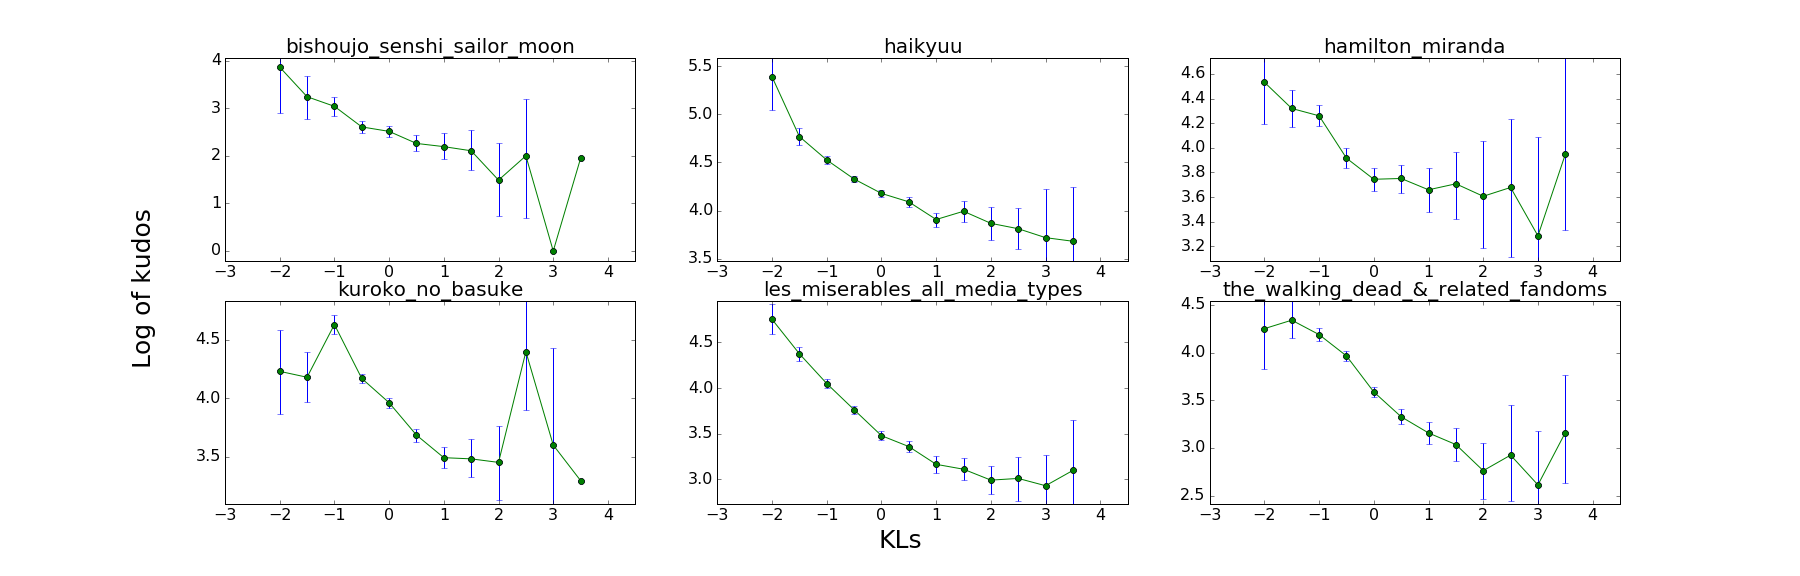
\includegraphics[width=1.1\textwidth]{/kl_kudos.png}
\caption{The Kudos fictions receive drop when the fictions' Kullback-Leibler divergence to the typical fictions in the corresponding time periods increase. Results from 6 fandoms are shown. The KL divergence are normalized into z-scores; the Kudos data are log-transformed. }
\end{center}
\end{figure}

\printbibliography
    
\end{document} %}}}
